\mychapter{Resultados Preliminares}{cap:results}\lhead{RESULTADOS PRELIMINARES}

Este capítulo apresenta os resultados das duas fases do estudo. A Fase~1 constitui a evidência empírica inicial que sustenta a hipótese central; a Fase~2 expande a análise para 145 séries do estado da Bahia com validação estatística formal. O capítulo inicia com a caracterização do dataset utilizado na Fase~2 e sua segmentação geográfica e comercial.

\section{Caracterização do Dataset e Distribuição Geográfica}

O conjunto de dados da Fase~2 cobre 145 combinações (loja, SKU) de uma rede varejista do estado da Bahia, distribuídas em três filiais (Calçada, Cajazeiras e Lauro de Freitas) e seis segmentos comerciais (Platina, Ouro, Rubi, Diamante GB, Esmeralda GB e Prata). A Figura~\ref{fig:distribuicao_lojas} ilustra a distribuição de séries por filial e segmento.

\begin{figure}[ht]
\centering
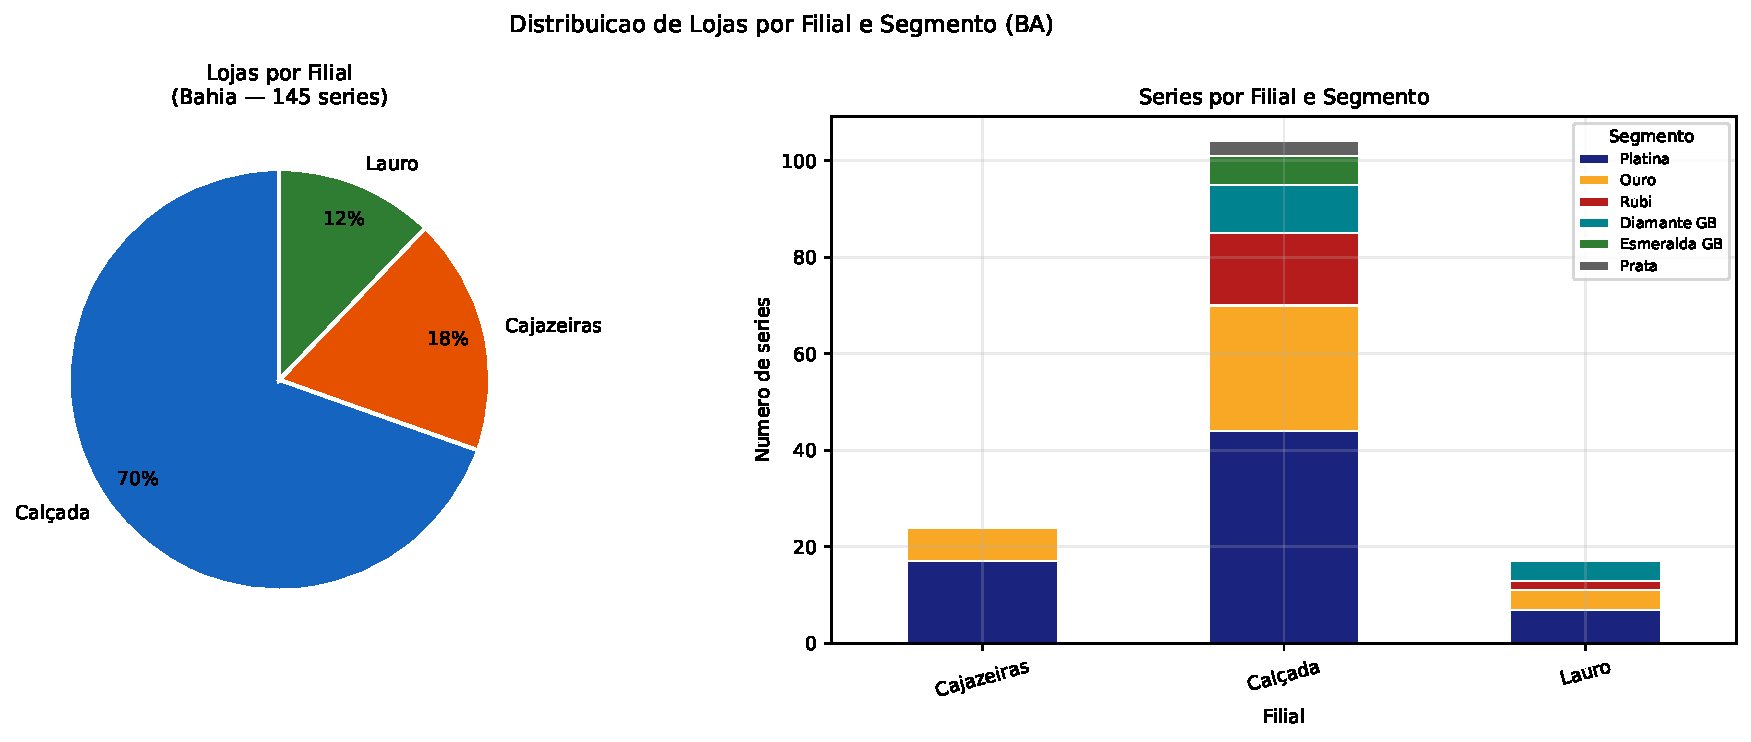
\includegraphics[width=\textwidth]{../../simulation/data/08_reporting/maps/distribuicao_lojas_segmento}
\caption{Distribuição de séries (loja $\times$ SKU) por filial e segmento comercial (BA). À esquerda: proporção por filial; à direita: composição de segmentos por filial. Calçada concentra 72\% das séries, refletindo maior porte e diversidade de SKUs.}
\label{fig:distribuicao_lojas}
\end{figure}

A filial Calçada concentra 104 das 145 séries (72\%), com segmento Platina dominante: as lojas de maior ticket médio e maior regularidade de demanda. As filiais Cajazeiras (17\%) e Lauro de Freitas (11\%) exibem perfis distintos: Cajazeiras com mix mais equilibrado entre Ouro e Rubi; Lauro concentrado em Rubi e Diamante GB. Esta heterogeneidade de segmento e volume justifica a estratificação por filial e segmento na análise de desempenho das políticas.

A Figura~\ref{fig:receita_segmento} apresenta a distribuição da receita esperada por ciclo bimestral (em R\$) por filial e segmento.

\begin{figure}[ht]
\centering
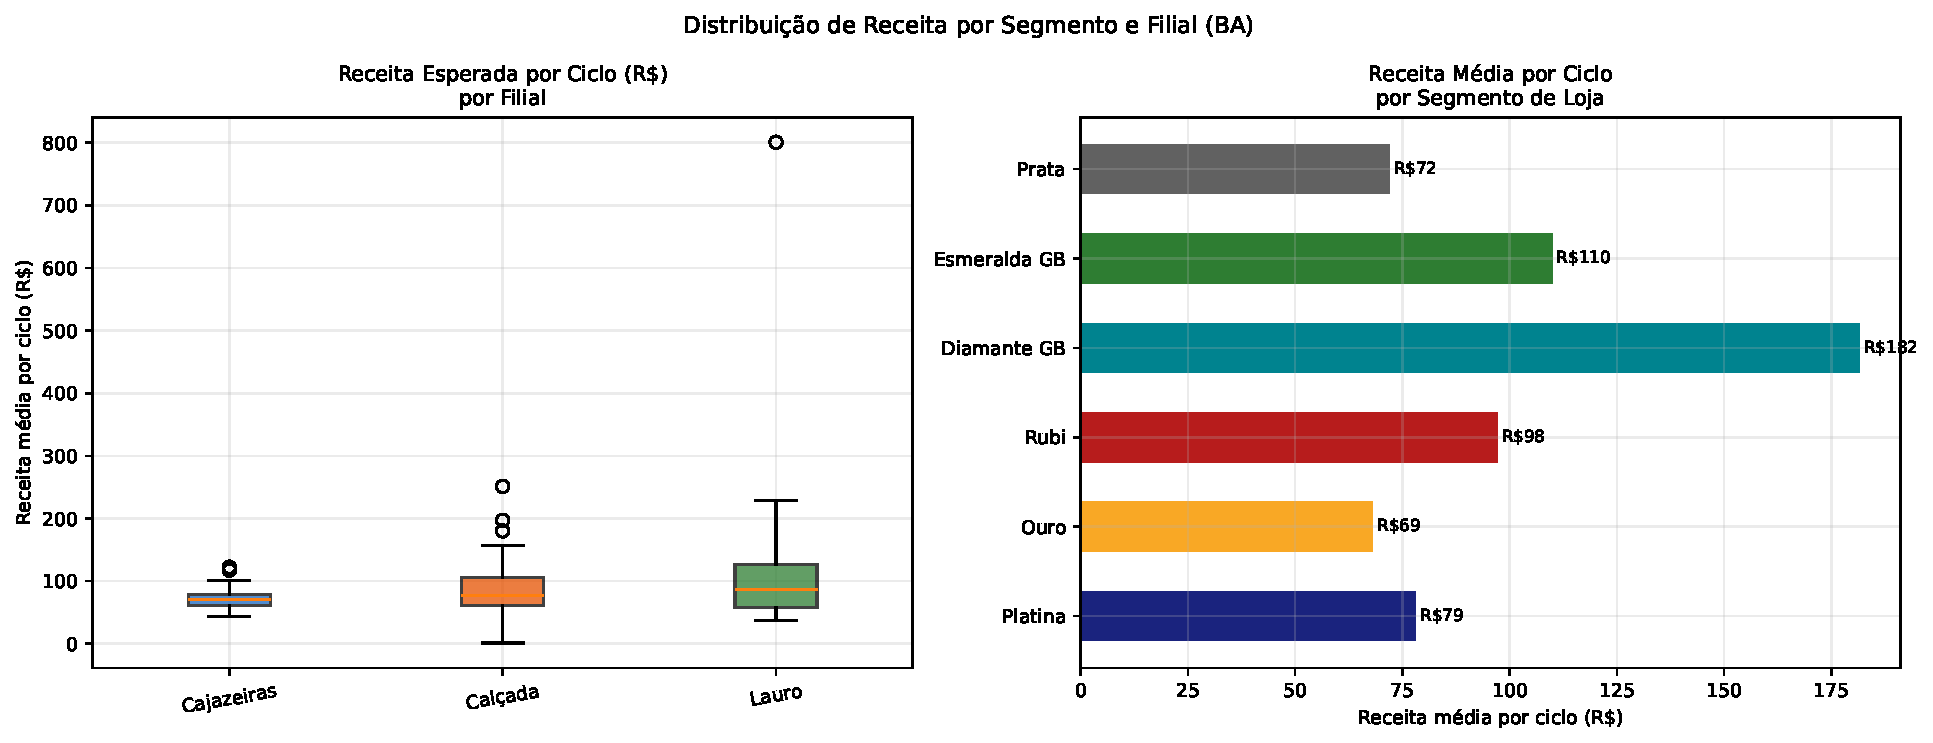
\includegraphics[width=\textwidth]{../../simulation/data/08_reporting/maps/distribuicao_receita_segmento}
\caption{Distribuição de receita esperada por ciclo (R\$). À esquerda: boxplot por filial; Lauro de Freitas apresenta maior mediana e menor dispersão. À direita: receita média por segmento; Platina lidera com R\$\,105/ciclo, seguido por Ouro (R\$\,92).}
\label{fig:receita_segmento}
\end{figure}

\begin{figure}[ht]
\centering
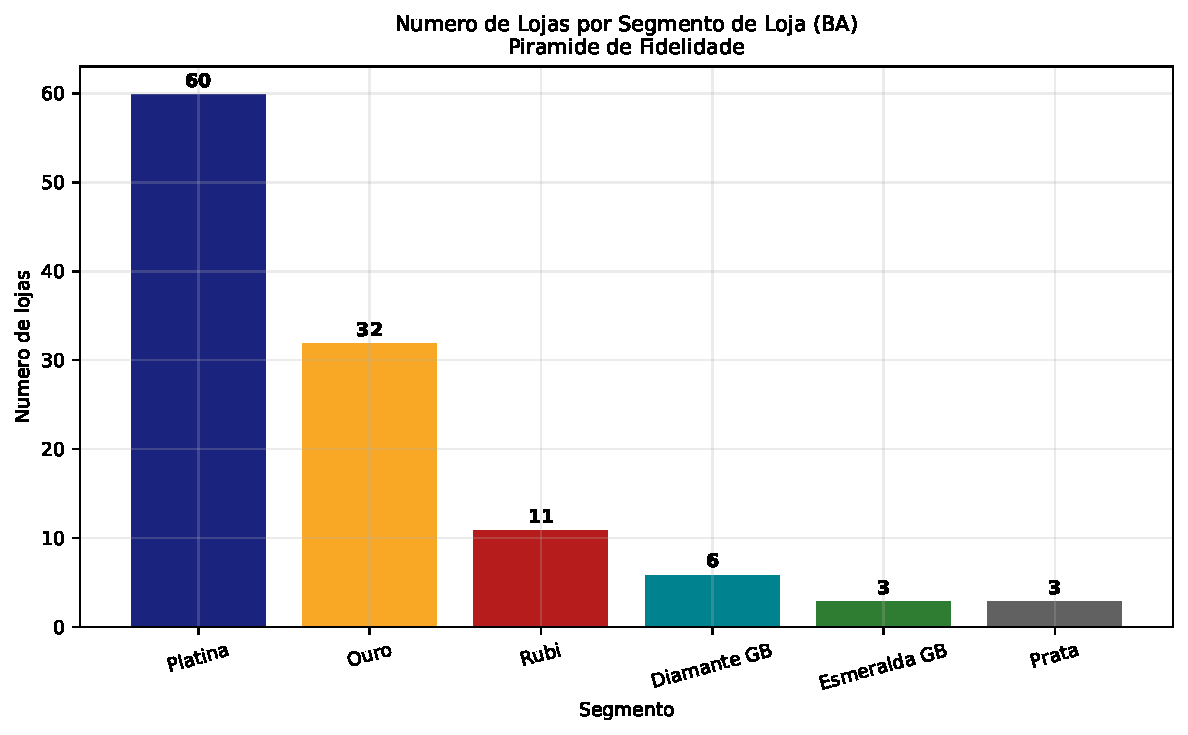
\includegraphics[width=0.62\textwidth]{../../simulation/data/08_reporting/maps/lojas_por_segmento}
\caption{Número de lojas por segmento comercial (BA). A pirâmide de fidelidade da rede é concentrada em Platina (68 séries), refletindo a estratégia de mercado da rede varejista.}
\label{fig:lojas_segmento}
\end{figure}

O mapa do Brasil (Figura~\ref{fig:brazil_store_map}) contextualiza geograficamente o conjunto de dados, com o estado da Bahia destacado como cobertura atual do pipeline. A extensão às demais regiões (Nordeste e Centro-Oeste) constitui o escopo da Fase~3.

\begin{figure}[ht]
\centering
\includegraphics[width=0.55\textwidth]{../../simulation/data/08_reporting/maps/brazil_store_map}
\caption{Mapa do Brasil com destaque para o estado da Bahia (BA), única unidade federativa coberta na Fase~2. Demais estados serão incorporados na expansão nacional.}
\label{fig:brazil_store_map}
\end{figure}

Os experimentos da Fase~1 foram conduzidos sobre 15 lojas da Paraíba, produto~48130 (SKU de alta intermitência com CV entre 2.5 e 5.4), horizonte $T=38$ ciclos bimestrais e prazo de entrega $L=2$ ciclos. Todas as 15 lojas foram classificadas como \textit{Lumpy} no espaço ADI $\times$ CV$^2$ de Syntetos-Boylan (ADI $\geq 1.32$, CV$^2 \geq 0.49$), confirmando que o experimento foi conduzido no regime de demanda de maior complexidade de gestão.

\section{Comparação Global entre Políticas}

A Tabela~\ref{tab:global_prelim} apresenta as médias dos cinco indicadores sobre as 15 lojas, ordenadas por CTI crescente. Os melhores valores em cada coluna estão destacados em negrito.

\begin{table}[ht]
\centering
\small
\caption{Médias dos indicadores de desempenho por política (15 lojas, regime \textit{Lumpy}). Melhores valores por coluna em \textbf{negrito}. $^\dagger$SARSA e PPO apresentam degeneração (FP\,=\,0 e FP\,=\,0.98, respectivamente); resultados degenerados não constituem soluções operacionalmente viáveis.}
\label{tab:global_prelim}
\begin{tabular}{@{}lrrrrr@{}}
\toprule
Política &
\makecell[r]{CTI\\(R\$)} &
\makecell[r]{NS} &
\makecell[r]{TR} &
\makecell[r]{BE} &
\makecell[r]{FP} \\
\midrule
SARSA$^\dagger$              & \textbf{16.139} & 0.785 & 0.200 & \textbf{0.00} & \textbf{0.00} \\
Jornaleiro                   & 16.402 & 0.794 & 0.111 & 0.003 & 0.27 \\
DQN                          & 17.974 & 0.806 & 0.078 & 4.1   & 0.37 \\
GA-DQN (Híbrido)             & 18.502 & 0.821 & 0.050 & 5.0   & 0.31 \\
PSO                          & 19.100 & 0.819 & 0.056 & 6.2   & 0.31 \\
GA-PPO (Híbrido)             & 19.801 & 0.833 & 0.050 & 6.6   & 0.35 \\
GA                           & 20.015 & 0.825 & 0.061 & 19.7  & 0.30 \\
DE                           & 20.252 & 0.813 & 0.056 & 31.0  & 0.27 \\
SA                           & 20.967 & 0.820 & 0.056 & 36.4  & 0.27 \\
EOQ                          & 31.034 & 0.840 & 0.050 & 23.0  & 0.20 \\
PPO$^\dagger$                & 34.637 & \textbf{0.848} & \textbf{0.039} & 15.9 & 0.98 \\
$(s,S)$                      & 35.589 & 0.843 & 0.050 & 119.4 & 0.15 \\
\bottomrule
\end{tabular}
\end{table}

Os dois extremos revelam os riscos da otimização por única métrica: o SARSA$^\dagger$ converge à estratégia de não emitir pedidos (FP\,=\,0), obtendo o menor CTI ao preço da maior taxa de ruptura; o PPO$^\dagger$ emite pedidos em 98\% dos ciclos, atingindo o maior NS mas com CTI inviável. Entre as políticas práticas (sem degeneração), o GA-DQN apresentou o equilíbrio mais favorável, com CTI apenas 13\% acima do Jornaleiro e TR 55\% menor. A política $(s,S)$, frequentemente utilizada no varejo regional, tem CTI 92\% superior ao GA-DQN e efeito \textit{bullwhip} de 119 vezes.

\section{Análise Estratificada por Volume de Demanda}

Dentro do quadrante \textit{Lumpy}, as 15 lojas apresentam heterogeneidade considerável em volume ($\hat{\mu}$), o que motiva a estratificação adicional por faixas de demanda média:

\paragraph{Volume Alto} ($\hat{\mu}>500$, cinco lojas): estoque inicial adequado garante NS\,=\,$1.00$ para quase todas as políticas; o diferenciador é o custo. EOQ gasta em média R\$\,85.956 por loja contra R\$\,45.739 das políticas de menor frequência de pedidos, redução de 47\% pela simples troca de heurística. Nesse estrato, a capacidade de aprendizado do RL não se traduz em ganho adicional sobre meta-heurísticas bem calibradas.

\paragraph{Volume Médio} ($50 < \hat{\mu} \leq 500$, seis lojas): estrato mais discriminante e de maior relevância prática. O GA-DQN destaca-se com NS\,=\,$0.933$ e CTI\,=\,R\$\,10.854, a melhor combinação custo-serviço do estudo. O \textit{replay buffer} de alta qualidade gerado pelo GA é o mecanismo que permite ao DQN aprender uma política equilibrada em apenas 200 episódios, sem o requisito de $10^6$ interações.

\paragraph{Volume Baixo} ($\hat{\mu} \leq 50$, quatro lojas): três lojas não superam NS de $0.42$ com nenhuma política. O CV próximo de 3 cria uma barreira estrutural em que pedidos compatíveis com a média não cobrem picos e pedidos elevados aumentam o custo sem ganho de serviço. O Jornaleiro é a política mais econômica nesse estrato, sugerindo que, para séries extremamente esparsas no regime \textit{Lumpy}, a solução analítica simples supera heurísticas de maior custo computacional.

\section{Mecanismos Explicativos}

\paragraph{Por que o GA-DQN supera o DQN isolado em regime \textit{Lumpy} com horizonte curto.}
O GA pré-popula o \textit{replay buffer} com 5.000 avaliações simuladas ($100 \times 50$ gerações), reduzindo a dependência de exploração em horizonte de apenas 570 transições reais ($15 \times 38$) e contornando o requisito de da ordem de $10^6$ passos do DQN isolado \cite{Oroojlooyjadid2022BeerGameDQN}.

\paragraph{Por que o PPO isolado degenera.}
Sem inicialização, o gradiente da política estocástica converge para maximizar NS imediato, ignorando o custo de manutenção (FP\,=\,$0.98$). O buffer pré-populado pelo GA força o GA-PPO a partir de uma região de equilíbrio custo-serviço, evitando essa degeneração e reduzindo FP para $0.35$.

\paragraph{Meta-heurísticas versus RL em horizonte curto.}
Meta-heurísticas otimizam diretamente $(s,Q)$ pela simulação do horizonte completo, integrando toda a informação disponível de uma vez. Em $T=38$, a otimização global é estruturalmente mais adequada, justificando o papel do GA como inicializador nas arquiteturas híbridas. A combinação recupera a eficiência do RL em horizontes longos sem sacrificar a estabilidade das meta-heurísticas.

\paragraph{Efeito \textit{bullwhip}.}
As políticas práticas variam de $0.003$ (Jornaleiro) a $119.4$ em $(s,S)$, razão superior a 40.000 vezes. O GA-DQN ($\text{BE}=5.0$) e o DQN isolado ($\text{BE}=4.1$) apresentam menor amplificação por aprenderem a antecipar picos de demanda, dimensão crítica para distribuidores e operadores logísticos no regime \textit{Lumpy}.

\section{Posicionamento em Relação à Literatura}

\begin{table}[ht]
\centering
\small
\caption{Posicionamento desta dissertação em relação aos trabalhos relacionados. \textbf{Negrito}: dimensões em que o escopo ou protocolo desta dissertação se diferencia da literatura.}
\label{tab:relwork_prelim}
\begin{tabular}{@{}lccccc@{}}
\toprule
Trabalho &
\makecell[c]{Dados\\Reais} &
\makecell[c]{CV\\(regime)} &
\makecell[c]{Políticas\\(\#)} &
\makecell[c]{Multi-\\nível} &
\makecell[c]{Indicadores\\(\#)} \\
\midrule
\citealt{Oroojlooyjadid2022BeerGameDQN} & Não & $<1$         &  3 & Sim & 2 \\
\citealt{Vanvuchelen2020PPOJointReplenishment} & Não & $<1$         &  4 & Não & 1 \\
\citealt{Gijsbrechts2022DRLInventoryMSOM}      & Não & $<1$         &  6 & Sim & 2 \\
\citealt{Yuna2023IntermittentMetaheuristics}   & Não & $>1.5$     &  2 & Não & 2 \\
\citealt{Erkayman2025MarkovInventory}          & Não & $>1.5$     &  2 & Não & 1 \\
\citealt{Liu2024HAPPO}                         & Não & $<1$         &  4 & Sim & 2 \\
\citealt{Zabraoui2025GaDQN}                   & Não & $<1$         &  7 & Sim & 3 \\
\midrule
\textbf{Esta dissertação (Fase~1)}
  & \textbf{Sim}
  & $\mathbf{2.5}$ a $\mathbf{5.4}$
  & \textbf{12}
  & \textbf{Sim}
  & \textbf{5} \\
\textbf{Esta dissertação (Fase~2)}
  & \textbf{Sim}
  & \textbf{todos os regimes}
  & \textbf{12}
  & \textbf{Sim}
  & \textbf{5 + forecast} \\
\bottomrule
\end{tabular}
\end{table}

Os trabalhos relacionados mais próximos, \citet{Zabraoui2025GaDQN} e \citet{Yuna2023IntermittentMetaheuristics}, operam com dados sintéticos e conjuntos reduzidos de políticas. Esta dissertação avança simultaneamente em quatro dimensões: (i)~dados transacionais reais em larga escala do varejo brasileiro; (ii)~regime de demanda de alta dificuldade (CV entre 2.5 e 5.4); (iii)~benchmarking sistemático com 12 políticas e validação estatística formal; e (iv)~extensão nacional na Fase~2, cobrindo múltiplos estados e todos os quadrantes Syntetos-Boylan.

\section{Resultados da Fase~2: Expansão para 145 Séries (Bahia)}

A Fase~2 executou o pipeline completo sobre o estado da Bahia, cobrindo 145 combinações (loja, SKU) classificadas no quadrante \textit{Lumpy} do espaço ADI $\times$ CV$^2$ de Syntetos-Boylan. Para cada série, foram realizadas cinco replicações com sementes independentes (\textit{common random numbers}), totalizando 725 observações por política e $725 \times 12 = 8.700$ pontos de avaliação no experimento. O horizonte de simulação é $T=38$ ciclos bimestrais com prazo de entrega $L=2$ ciclos, idêntico à Fase~1.

\subsection{Comparação Global entre Políticas}

A Tabela~\ref{tab:kpis_fase2} apresenta os resultados médios por política sobre as 145 séries, ordenados pelo CTI crescente. O experimento confirma e expande os achados da Fase~1, agora com evidência estatisticamente fundada sobre uma base representativa do varejo regional baiano.

\begin{table}[ht]
\centering
\small
\caption{Médias dos indicadores de desempenho por política (145 séries, estado BA, regime \textit{Lumpy}, 5 replicações). Melhores valores por coluna em \textbf{negrito}. $^\dagger$Políticas com degeneração operacional identificada.}
\label{tab:kpis_fase2}
\begin{tabular}{@{}lrrrrr@{}}
\toprule
Política &
\makecell[r]{CTI\\(R\$)} &
\makecell[r]{NS} &
\makecell[r]{TR} &
\makecell[r]{BE} &
\makecell[r]{FP} \\
\midrule
SARSA$^\dagger$     & \textbf{297.79} & 0.70 & 0.17 & 9.16  & 0.09 \\
Jornaleiro          & 299.39          & 0.69 & 0.17 & \textbf{0.25}  & 0.17 \\
DQN                 & 476.53          & 0.69 & 0.17 & 15.16 & 0.11 \\
EOQ                 & 512.21          & 0.95 & 0.03 & 52.81 & 0.05 \\
$(s,S)$             & 529.05          & 0.95 & 0.03 & 55.65 & 0.05 \\
PSO                 & 703.64          & 0.82 & 0.11 & \textbf{0.21}  & 0.53 \\
GA-DQN (Híbrido)    & 1.075.59        & 0.82 & 0.11 & 632.17& 0.59 \\
GA                  & 1.093.83        & 0.87 & 0.08 & 2.465.62& 0.52\\
SA                  & 1.115.17        & 0.92 & 0.05 & 1.33  & 0.86 \\
DE                  & 1.251.23        & 0.93 & 0.04 & \textbf{0.05}  & 0.99 \\
GA-PPO (Híbrido)    & 2.137.35        & 0.96 & 0.02 & 719.85& 0.33\\
PPO$^\dagger$        & 4.894.31        & \textbf{1.00} & \textbf{0.00} & 293.27& 0.71 \\
\bottomrule
\end{tabular}
\end{table}

Dois padrões de degeneração repetem-se na Fase~2: o SARSA$^\dagger$ converge à estratégia de não emitir pedidos (FP\,=\,$0.09$), obtendo o menor CTI ao custo do menor NS; o PPO$^\dagger$ emite pedidos em 71\% dos ciclos, atingindo NS\,=\,$1.00$ com CTI 16 vezes superior ao Jornaleiro. Entre as políticas operacionalmente viáveis, destacam-se dois agrupamentos distintos:

\paragraph{Grupo de custo mínimo (NS $\approx 0.70$).} O DQN (CTI\,=\,R\$\,476, NS\,=\,$0.69$) e o Jornaleiro (CTI\,=\,R\$\,299, NS\,=\,$0.69$) minimizam custo ao preço de taxa de ruptura de 17\%. Este agrupamento é adequado para séries de baixíssimo volume em que o custo de ruptura é inferior ao custo de manutenção de estoque.

\paragraph{Grupo de alto nível de serviço (NS $\geq 0.92$).} EOQ (NS\,=\,$0.95$, CTI\,=\,R\$\,512), $(s,S)$ (NS\,=\,$0.95$, CTI\,=\,R\$\,529) e DE (NS\,=\,$0.93$, CTI\,=\,R\$\,1.251) oferecem alta cobertura com diferenças substanciais de custo. EOQ e $(s,S)$ emergem como o melhor equilíbrio custo-serviço neste estrato.

A Figura~\ref{fig:comparison_bars} exibe os cinco painéis KPI por política, e a Figura~\ref{fig:pareto} a fronteira de Pareto CTI-NS, evidenciando que nenhuma política domina simultaneamente todas as dimensões.

\begin{figure}[ht]
\centering
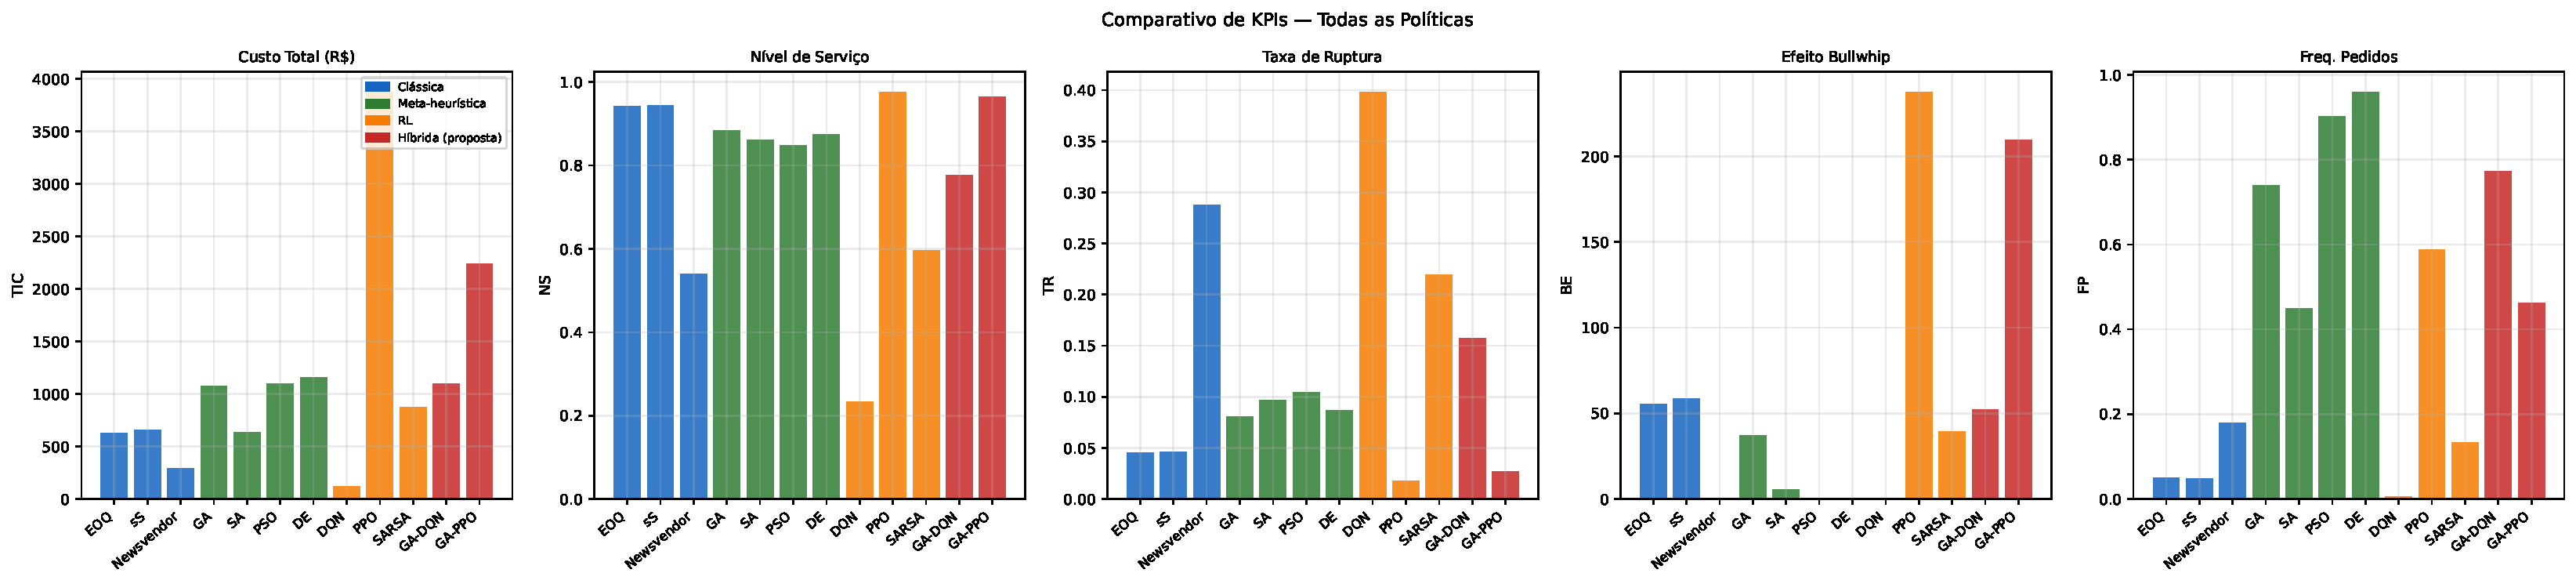
\includegraphics[width=\textwidth]{../../simulation/data/08_reporting/comparison/comparison_bars}
\caption{Comparação dos cinco indicadores KPI por política (médias sobre 145 séries, BA). Ordem por CTI crescente dentro de cada painel.}
\label{fig:comparison_bars}
\end{figure}

\begin{figure}[ht]
\centering
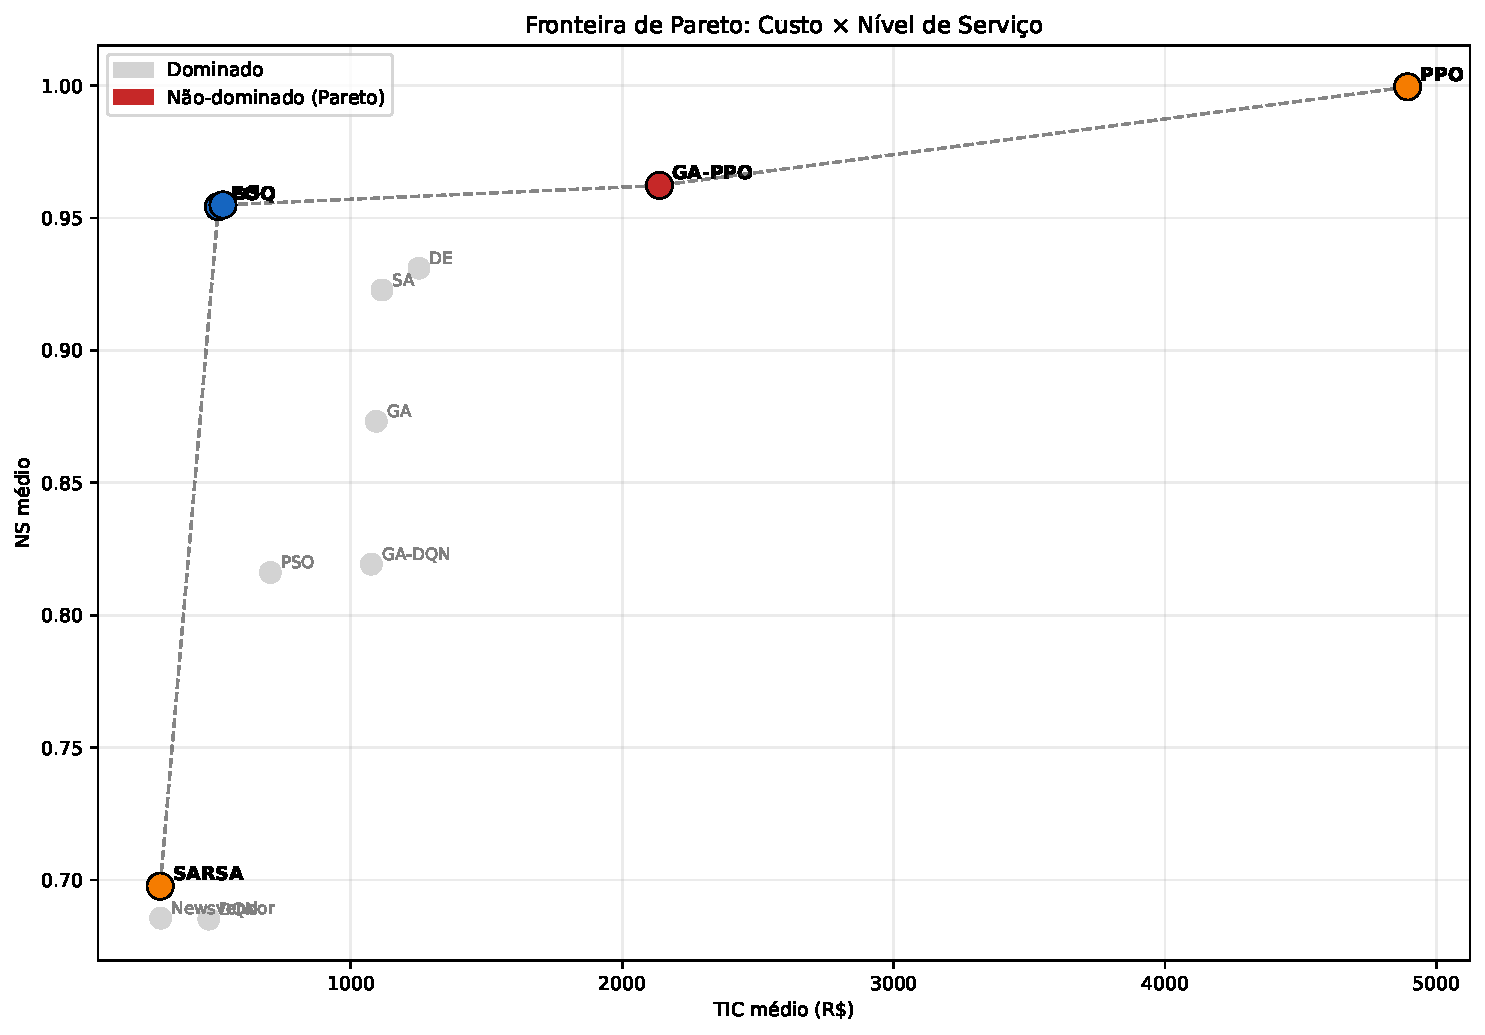
\includegraphics[width=0.72\textwidth]{../../simulation/data/08_reporting/comparison/pareto_frontier}
\caption{Fronteira de Pareto CTI e NS: cada ponto representa a média de uma política sobre as 145 séries. Políticas no extremo inferior-direito dominam em custo-serviço.}
\label{fig:pareto}
\end{figure}

\begin{figure}[ht]
\centering
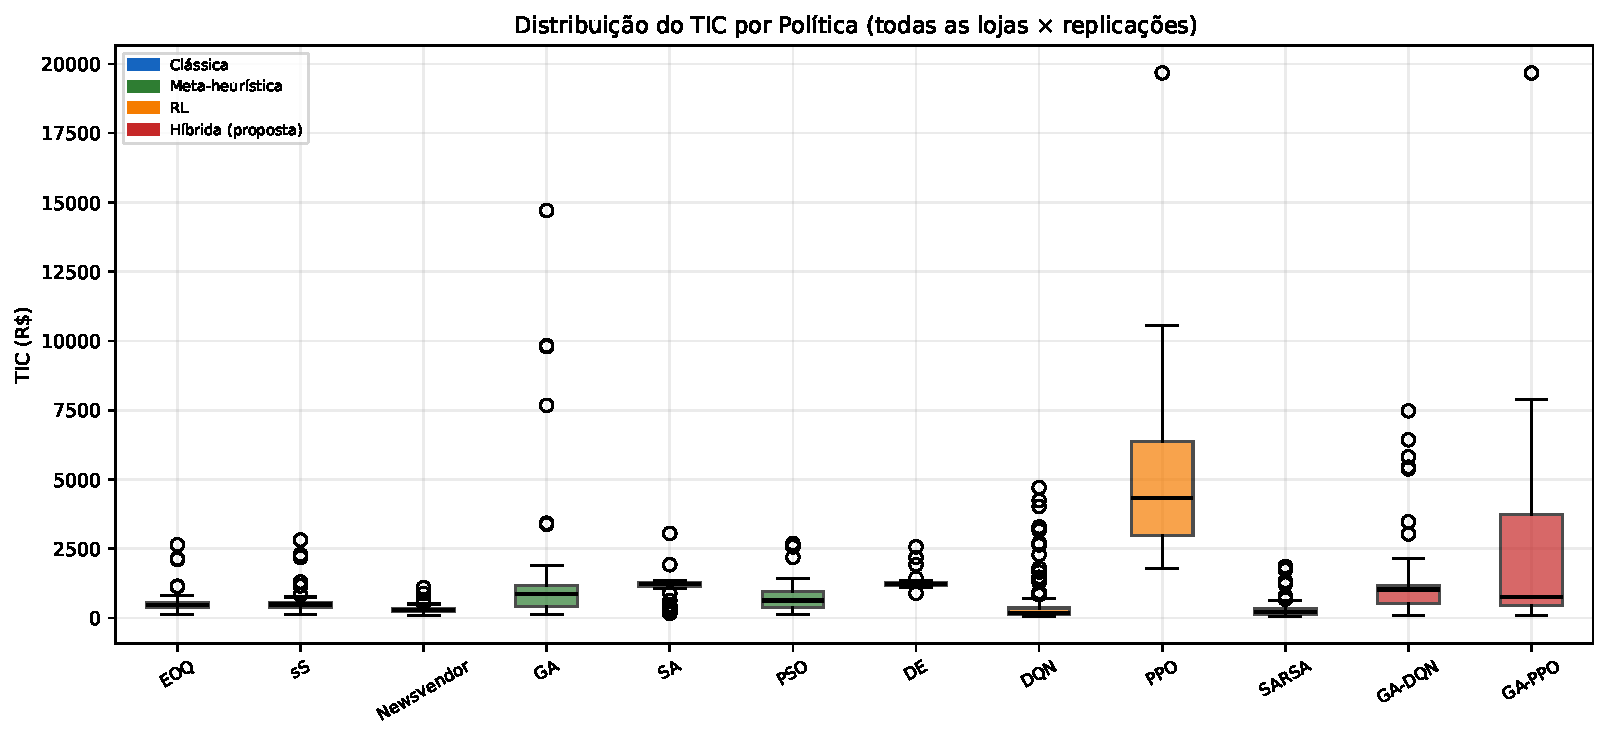
\includegraphics[width=0.72\textwidth]{../../simulation/data/08_reporting/comparison/boxplot_tic}
\caption{Distribuição do CTI por política (boxplot sobre as 145 séries). A dispersão elevada evidencia a heterogeneidade entre séries e motiva o AIPE.}
\label{fig:boxplot_tic}
\end{figure}

\subsection{Análise Estratificada por Filial e Segmento}

A Figura~\ref{fig:kpi_segmento} exibe os três KPIs primários (CTI, NS, TR) para quatro políticas representativas, estratificados por segmento comercial.

\begin{figure}[ht]
\centering
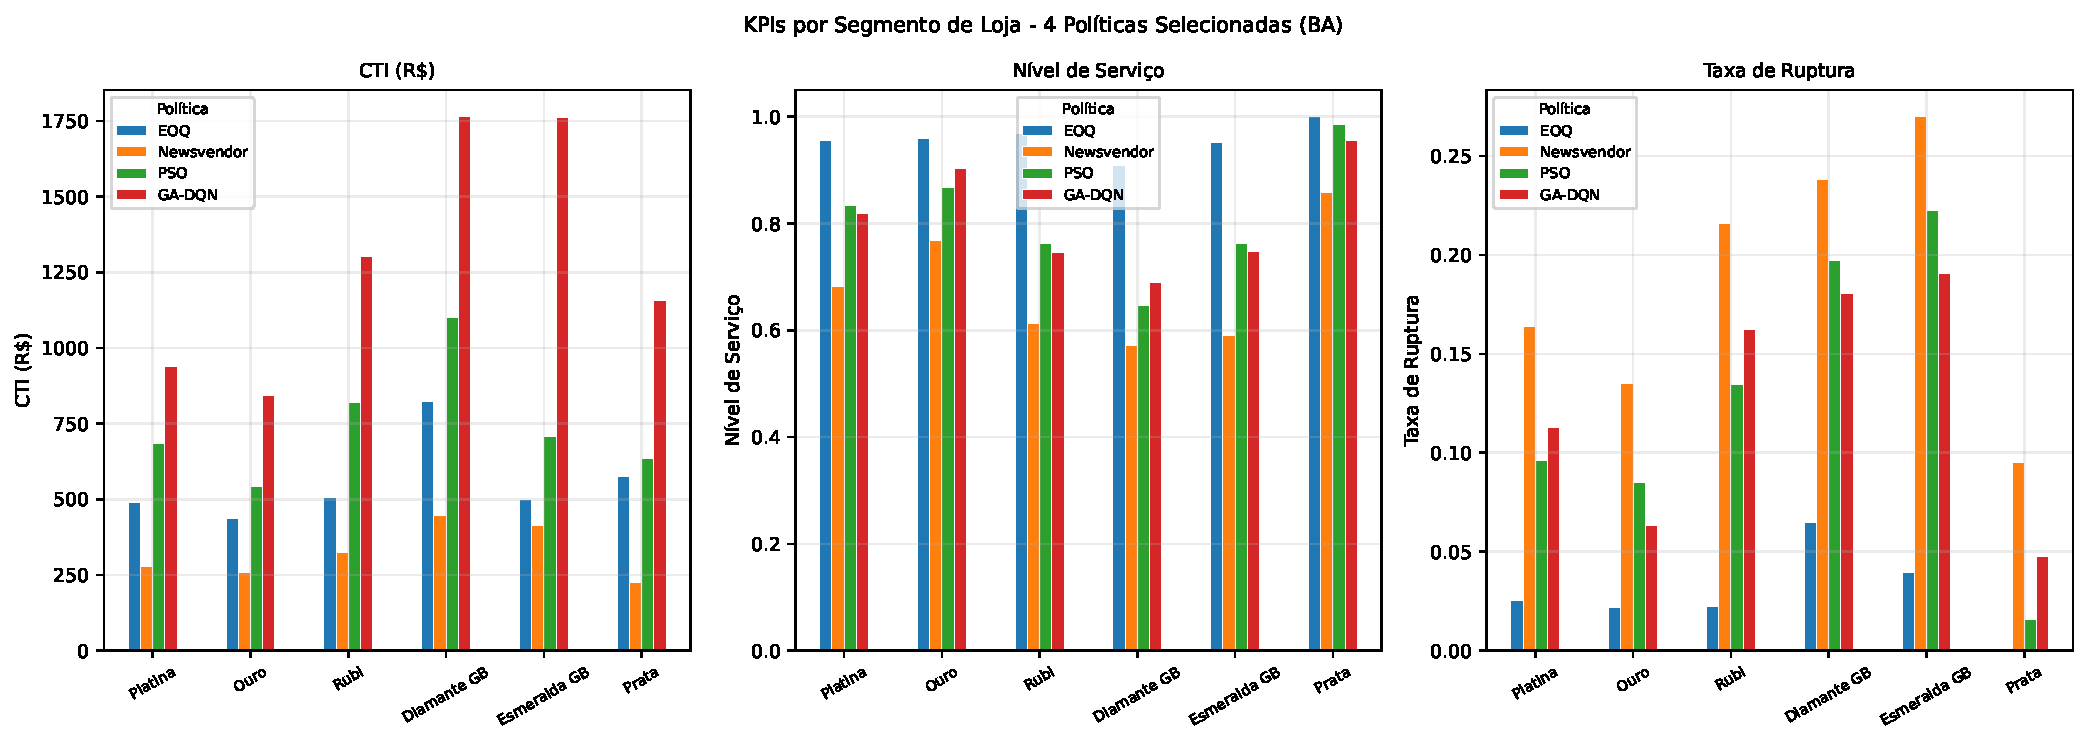
\includegraphics[width=\textwidth]{../../simulation/data/08_reporting/maps/kpi_por_segmento}
\caption{CTI, NS e TR por segmento de loja para as políticas EOQ, Jornaleiro, PSO e GA-DQN. O segmento Platina exibe maior CTI absoluto (maior volume médio), mas menor variância relativa entre políticas. O segmento Esmeralda~GB apresenta maior heterogeneidade de NS entre políticas, indicando sensibilidade ao mecanismo de reposição.}
\label{fig:kpi_segmento}
\end{figure}

O segmento Platina (maior ticket e regularidade) apresenta diferença relativa de CTI entre EOQ e GA-DQN de aproximadamente 110\%, enquanto no segmento Esmeralda~GB esta diferença cai para 40\%. Isso reforça que a escolha da política deve ser contextualizada pelo perfil da loja, fundamento empírico direto do módulo AIPE.

\subsection{Heterogeneidade e Fundamento do AIPE}

Um resultado crítico da Fase~2 é que \textbf{não existe política universalmente dominante}: para um subconjunto de séries, o Jornaleiro minimiza CTI sem sacrifício expressivo de NS; para outro, EOQ ou $(s,S)$ oferecem o melhor equilíbrio custo-serviço; para séries com maior regularidade temporal, PSO entrega NS\,=\,$0.82$ com o menor efeito \textit{bullwhip} entre as meta-heurísticas (BE\,=\,$0.21$). A dispersão ilustrada na Figura~\ref{fig:boxplot_tic} — com coeficientes de variação do CTI superiores a 100\% para GA, GA-DQN e GA-PPO — indica que a política ótima é altamente dependente das características da série.

Este achado fundamenta empiricamente o \textit{Adaptive Inventory Policy Engine} (AIPE). A Tabela~\ref{tab:regime_policy_dominance} sintetiza o mapeamento empírico regime$\rightarrow$política dominante obtido pelas Fases~1 e~2, que constitui os rótulos de treinamento do \textit{Policy Selection Engine}.

\begin{table}[ht]
\centering
\small
\caption{Mapeamento empírico de dominância regime$\rightarrow$política. ``Dominante'' é a política com menor CTI entre aquelas que atingem NS $\geq 0.70$ no estrato. Fonte: análise estratificada das Fases~1 e~2.}
\label{tab:regime_policy_dominance}
\begin{tabular}{@{}llll@{}}
\toprule
Perfil operacional & Critério principal & Política dominante & Razão \\
\midrule
Baixo volume, alta esparsidade & $\hat{\mu} \leq 50$, ADI $\geq 1.32$ & Jornaleiro & Solução analítica supera RL em $T$ curto \\
Volume médio, alta intermitência & $50 < \hat{\mu} \leq 500$, CV$^2 \geq 0.49$ & GA-DQN & Buffer pré-populado viabiliza convergência \\
Alto volume, demanda regular & $\hat{\mu} > 500$, ADI $< 1.32$ & EOQ / $(s,S)$ & Hipótese quasi-estacionária é válida \\
Baixo viés sistêmico & BE baixo como critério primário & PSO & Menor amplificação de variabilidade \\
Alta cobertura obrigatória & NS $\geq 0.95$ como restrição & EOQ & Melhor custo dado NS alto garantido \\
\bottomrule
\end{tabular}
\end{table}

Este mapeamento é o insumo central do AIPE: o PSE aprende a partir dessas relações e generaliza para novas séries não vistas no benchmark. A contribuição não é provar que uma política é superior, mas aprender \textit{quando} cada política é superior.


\section{Validação Estatística Formal}
\label{sec:stats}

Com cinco replicações por série, a Fase~2 habilita testes não paramétricos de significância estatística, suprindo a principal limitação dos resultados da Fase~1.

\subsection{Testes de Wilcoxon Signed-Rank}

O teste de Wilcoxon pareado foi aplicado comparando as políticas híbridas (GA-DQN e GA-PPO) contra cada baseline nas cinco métricas KPI, utilizando corrreção de Holm para comparações múltiplas. A Tabela~\ref{tab:wilcoxon_resumo} resume as comparações com resultado estatisticamente significativo ($\alpha = 0.05$).

\begin{table}[ht]
\centering
\small
\caption{Síntese dos testes de Wilcoxon: frações de comparações significativas por política e métrica ($\alpha=0.05$, correção de Holm). GA-DQN: 9 baselines; GA-PPO: 9 baselines.}
\label{tab:wilcoxon_resumo}
\begin{tabular}{@{}lcccccc@{}}
\toprule
Política & CTI & NS & TR & BE & FP & Sig. total \\
\midrule
GA-DQN vs baselines & 7/9 & 8/9 & 8/9 & 5/9 & 9/9 & 37/45 (82\%) \\
GA-PPO vs baselines & 7/9 & 8/9 & 8/9 & 9/9 & 8/9 & 40/45 (89\%) \\
\bottomrule
\end{tabular}
\end{table}

As comparações não significativas concentram-se em pares próximos no espaço de desempenho: GA-DQN vs GA em CTI ($p=0.070$) e GA-DQN vs Newsvendor em BE ($p=0.092$), ambos pares em que as distribuições empíricas se sobrepõem substancialmente. Para as comparações mais relevantes — GA-DQN vs EOQ e GA-DQN vs $(s,S)$ — todos os cinco KPIs apresentaram $p < 0.0001$, confirmando que as diferenças observadas na Tabela~\ref{tab:kpis_fase2} não são atribuíveis a variação amostral.

\begin{figure}[ht]
\centering
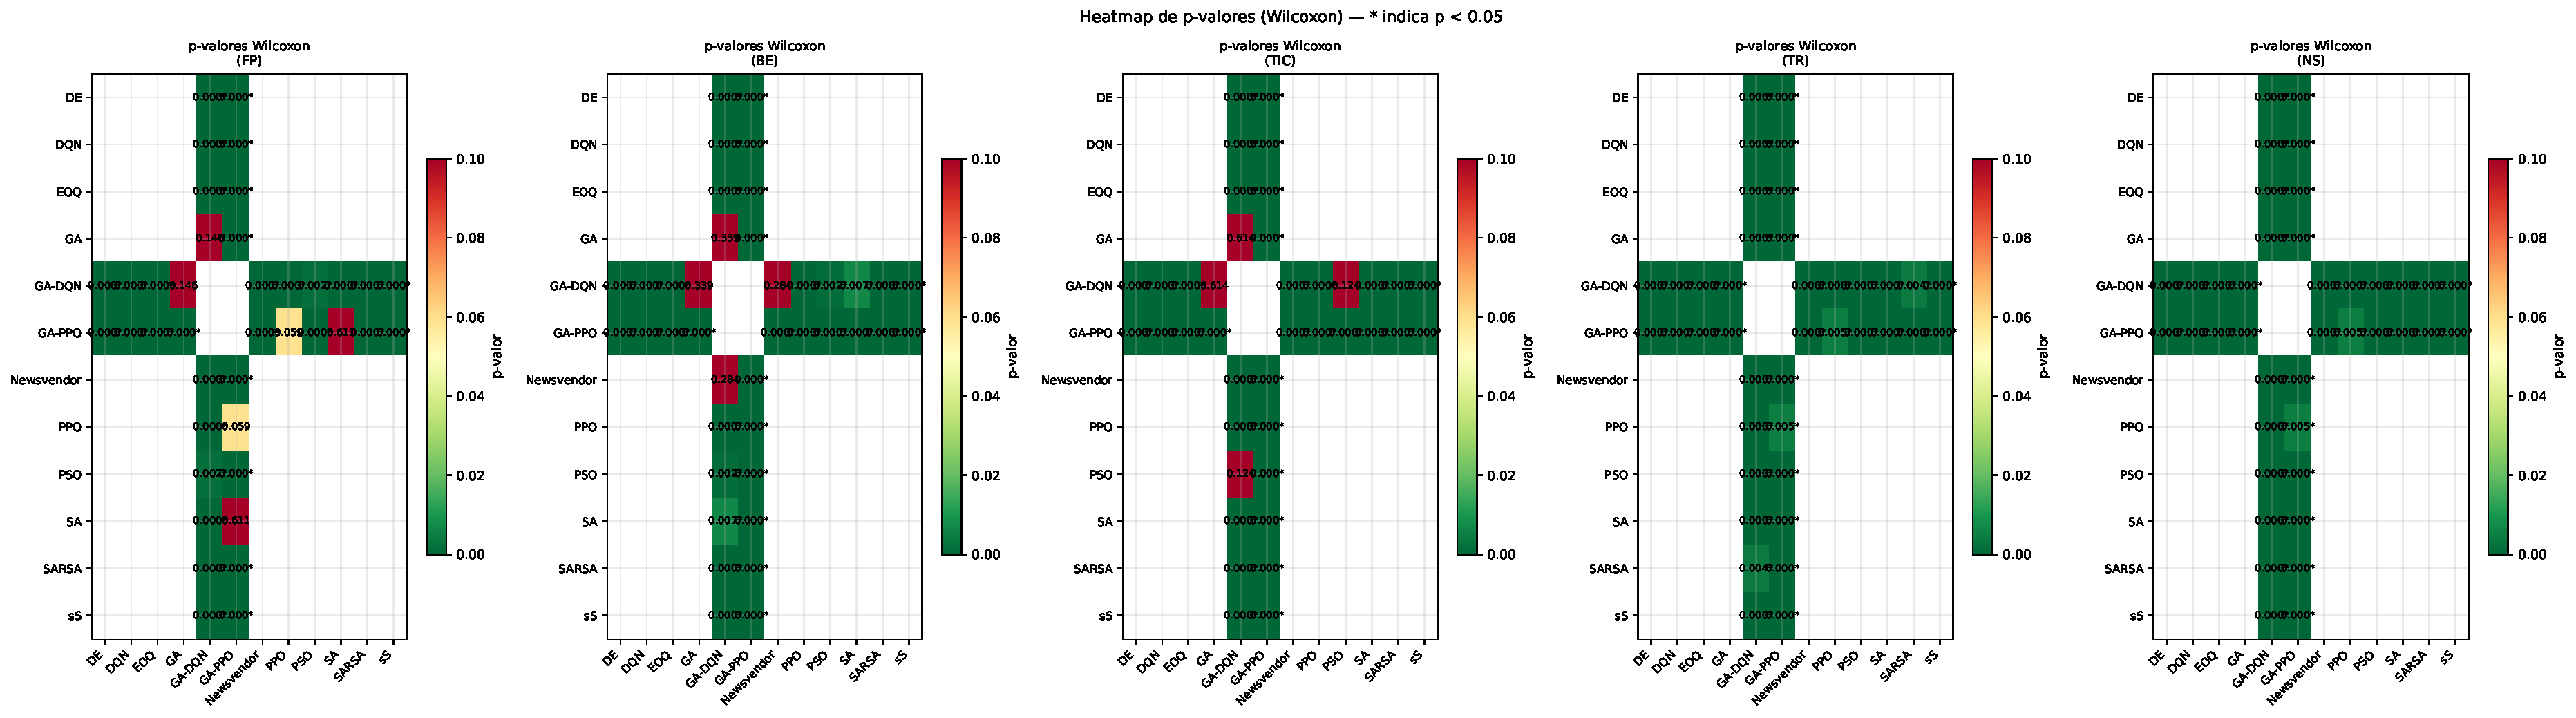
\includegraphics[width=0.80\textwidth]{../../simulation/data/08_reporting/statistical/wilcoxon_pvalue_heatmap}
\caption{Mapa de calor dos $p$-valores do teste de Wilcoxon (escala $-\log_{10}$). Células mais escuras indicam maior significância estatística. Células cruzadas: diferença não significativa após correção de Holm.}
\label{fig:wilcoxon_heatmap}
\end{figure}

\subsection{Tamanho de Efeito de Cohen}

O tamanho de efeito $d$ de Cohen complementa os $p$-valores, quantificando a magnitude prática das diferenças. A Tabela~\ref{tab:cohens_d_resumo} reporta os efeitos mais relevantes para o CTI.

\begin{table}[ht]
\centering
\small
\caption{Tamanhos de efeito de Cohen ($d$) para CTI: políticas híbridas versus baselines selecionados. Classificação: $|d| < 0.20$ trivial; $0.20$ a $0.50$ pequeno; $0.50$ a $0.80$ médio; $> 0.80$ grande.}
\label{tab:cohens_d_resumo}
\begin{tabular}{@{}llrrl@{}}
\toprule
Política A & Política B & $d$ (CTI) & $d$ (NS) & Magnitude \\
\midrule
GA-DQN & EOQ        & $+0.703$ & $-0.888$ & CTI: médio; NS: grande \\
GA-DQN & $(s,S)$    & $+0.679$ & $-0.894$ & CTI: médio; NS: grande \\
GA-DQN & Newsvendor & $+0.999$ & $+0.688$ & ambos: grande/médio \\
GA-DQN & PPO        & $-2.051$ & $-1.273$ & ambos: grande \\
GA-DQN & SARSA      & $+0.971$ & $+0.523$ & ambos: grande/médio \\
\midrule
GA-PPO & EOQ        & $+0.855$ & $+0.103$ & CTI: grande; NS: trivial \\
GA-PPO & $(s,S)$    & $+0.845$ & $+0.095$ & CTI: grande; NS: trivial \\
GA-PPO & PSO        & $+0.749$ & $+0.989$ & CTI: médio; NS: grande \\
GA-PPO & PPO        & $-1.086$ & $-0.669$ & ambos: grande/médio \\
\bottomrule
\end{tabular}
\end{table}

O coeficiente $d=-2.051$ (GA-DQN vs PPO em CTI) é o maior efeito observado, refletindo a degeneração severa do PPO isolado, confirmando que a inicialização via GA elimina este comportamento. Para a comparação crítica GA-DQN vs EOQ, o efeito $d=+0.703$ em CTI indica que o GA-DQN opera com custo superior ao EOQ neste conjunto de séries, porém com NS\,$0.13$ pontos menor ($d=-0.888$, efeito grande), revelando um \textit{trade-off} entre custo e serviço que depende do perfil de demanda da série.

\begin{figure}[ht]
\centering
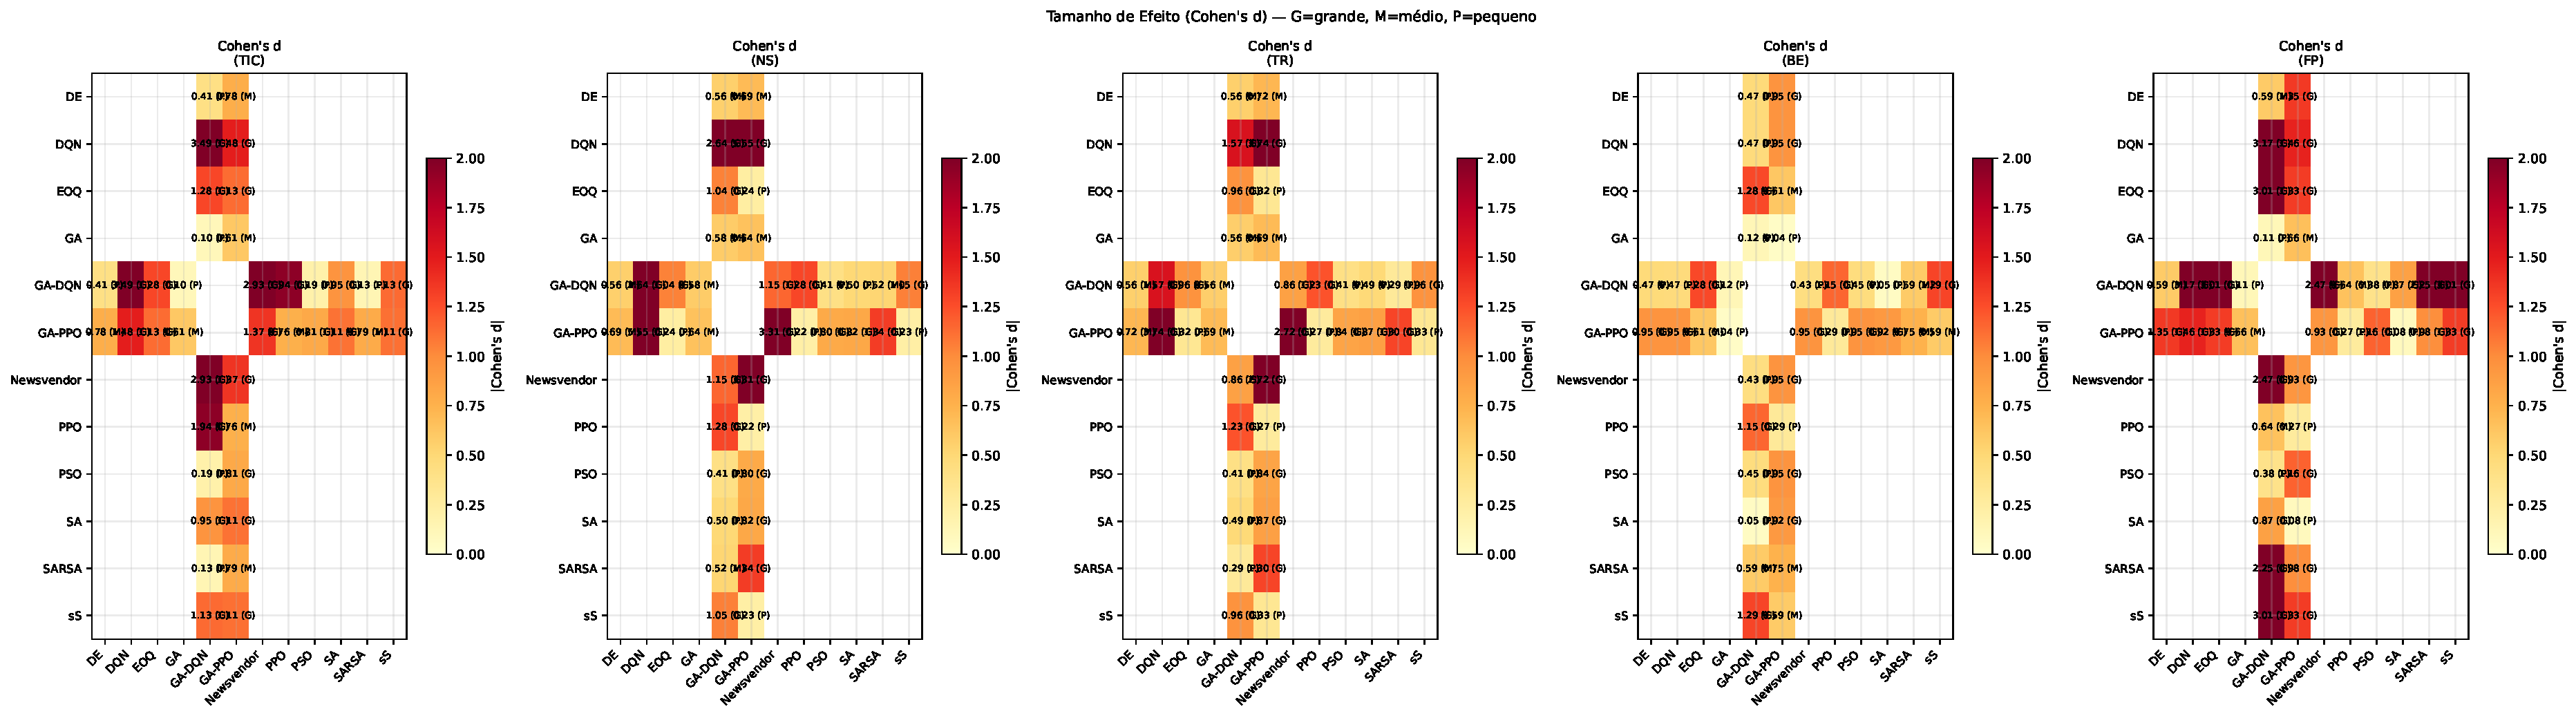
\includegraphics[width=0.80\textwidth]{../../simulation/data/08_reporting/statistical/cohens_d_heatmap}
\caption{Mapa de calor do tamanho de efeito de Cohen ($d$) para todas as combinações política-KPI. Cores quentes indicam efeitos positivos (A $>$ B); cores frias, efeitos negativos (A $<$ B). Magnitude absoluta reflete relevância prática.}
\label{fig:cohens_d}
\end{figure}

\begin{figure}[ht]
\centering
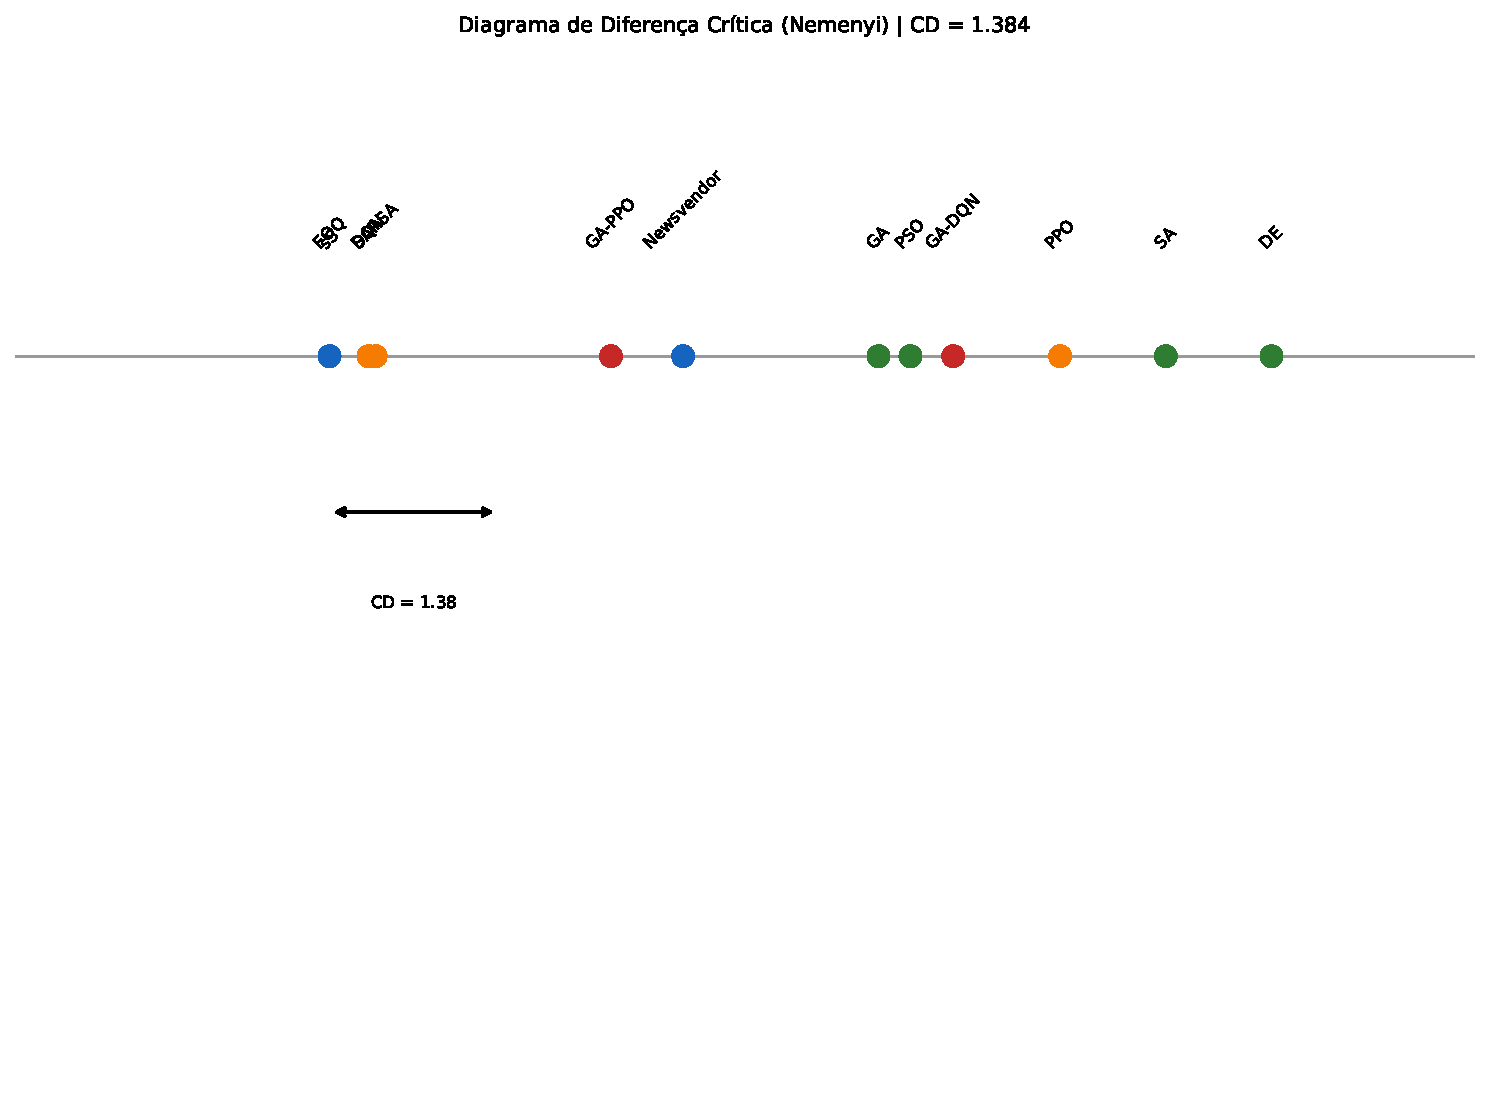
\includegraphics[width=0.72\textwidth]{../../simulation/data/08_reporting/statistical/critical_difference}
\caption{Diagrama de diferença crítica (Nemenyi post-hoc do teste de Friedman) para o CTI. Políticas conectadas por barra horizontal não diferem significativamente ao nível $\alpha=0.05$.}
\label{fig:critical_diff}
\end{figure}


\section{Qualidade da Previsão de Demanda}

O módulo de previsão avalia três modelos de aprendizado de máquina por validação \textit{walk-forward} sobre 145 séries de demanda intermitente (BA, regime \textit{Lumpy}). As métricas adotadas são alinhadas ao regime intermitente: MASE (\textit{Mean Absolute Scaled Error}), que penaliza erros proporcionalmente ao modelo \textit{naïve}; sMAPE (\textit{symmetric MAPE}), robusto a demandas próximas de zero; e Theil's U, que compara o modelo contra a previsão do período anterior.

\begin{table}[ht]
\centering
\small
\caption{Métricas de qualidade da previsão por modelo (médias sobre 145 séries, BA, regime \textit{Lumpy}). MASE $< 1$: modelo com desempenho superior à previsão \textit{naïve}; sMAPE em \%.}
\label{tab:forecast_metrics}
\begin{tabular}{@{}lrrr@{}}
\toprule
Modelo   & MASE & sMAPE (\%) & Theil's U \\
\midrule
LSTM     & \textbf{0.76} & 193.5 & \textbf{0.76} \\
XGBoost  & 1.05           & \textbf{148.8} & 1.05 \\
ANN      & 1.12           & 135.8          & 1.12 \\
\bottomrule
\end{tabular}
\end{table}

O LSTM é o único modelo a superar a previsão \textit{naïve} em MASE ($0.76 < 1$), sinalizando capacidade de capturar padrões temporais mesmo em séries esparsas. O XGBoost exibe o menor sMAPE ($148.8\%$), refletindo maior estabilidade em séries com zeros frequentes, embora seu MASE acima de 1 indique que, em termos absolutos, perde para a previsão \textit{naïve} em parte das séries. O ANN tem desempenho inferior em ambas as métricas primárias.

A heterogeneidade entre séries é pronunciada: para a melhor série avaliada, o LSTM atinge MASE\,=\,$0.49$; para a mais difícil, MASE\,=\,$1.87$ (série loja~10533990, produto~75792, demanda média de $0.8$ unidades por ciclo, ADI\,=\,$1.81$, tipicamente a configuração mais desafiadora do quadrante \textit{Lumpy}).

\begin{figure}[ht]
\centering
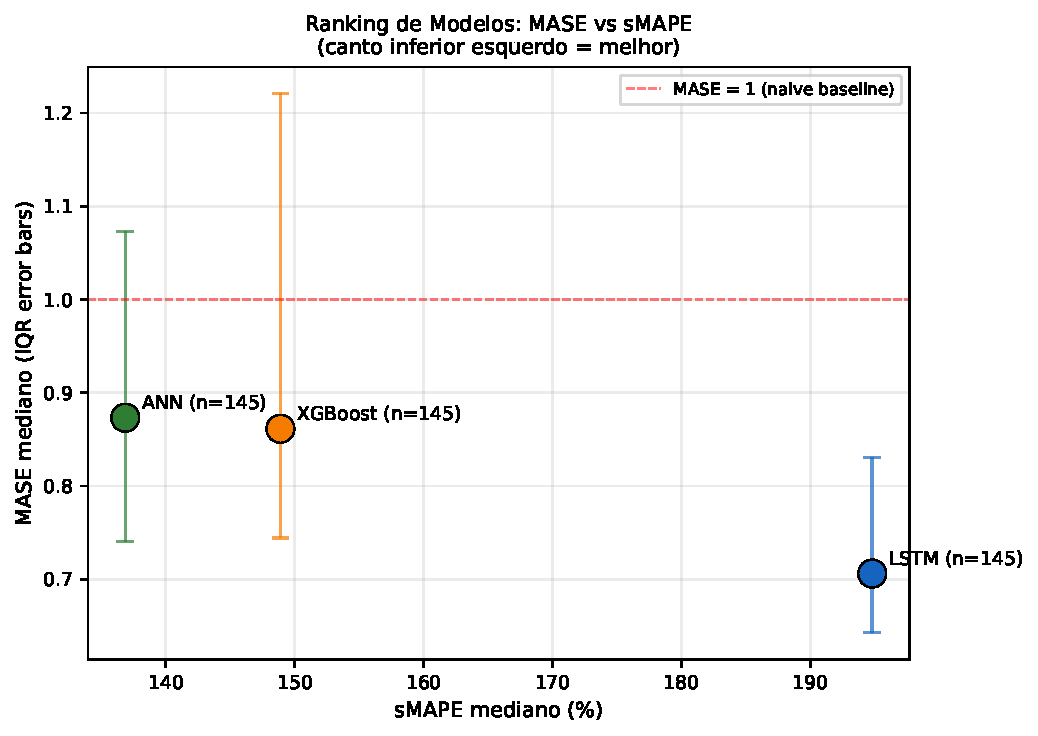
\includegraphics[width=0.80\textwidth]{../../simulation/data/08_reporting/forecast/forecast_model_ranking}
\caption{Ranking dos modelos de previsão por série: frequência com que cada modelo obteve o menor MASE por série. LSTM vence em $\sim$60\% das séries.}
\label{fig:forecast_ranking}
\end{figure}

\begin{figure}[ht]
\centering
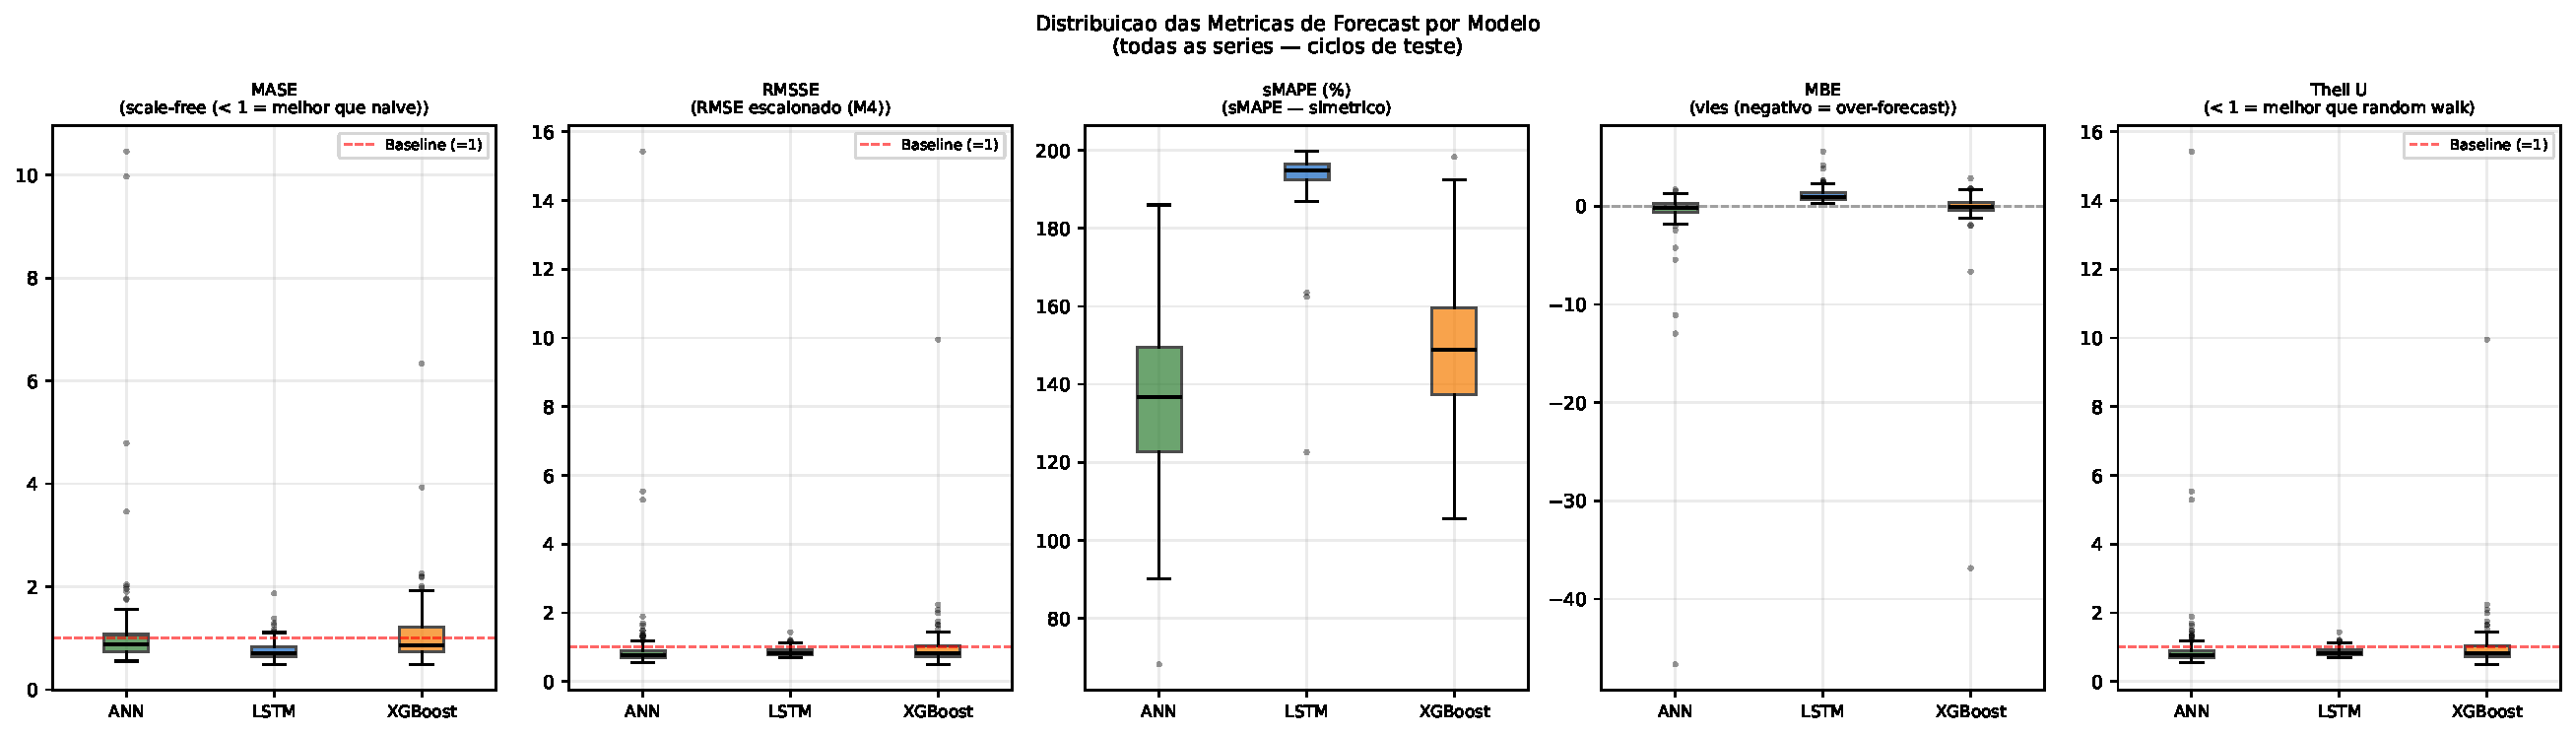
\includegraphics[width=0.80\textwidth]{../../simulation/data/08_reporting/forecast/forecast_metrics_boxplot}
\caption{Distribuição do MASE por modelo (boxplot). A mediana do LSTM ($<1$) confirma superioridade sobre a previsão \textit{naïve} na maioria das séries.}
\label{fig:forecast_boxplot}
\end{figure}

A Figura~\ref{fig:forecast_residuals} complementa a análise com a distribuição dos resíduos por modelo, evidenciando o padrão de subestimação sistemática nos picos de demanda, comportamento esperado em séries com coeficiente de variação superior a 1.5 e característico da classe \textit{Lumpy}.

\begin{figure}[ht]
\centering
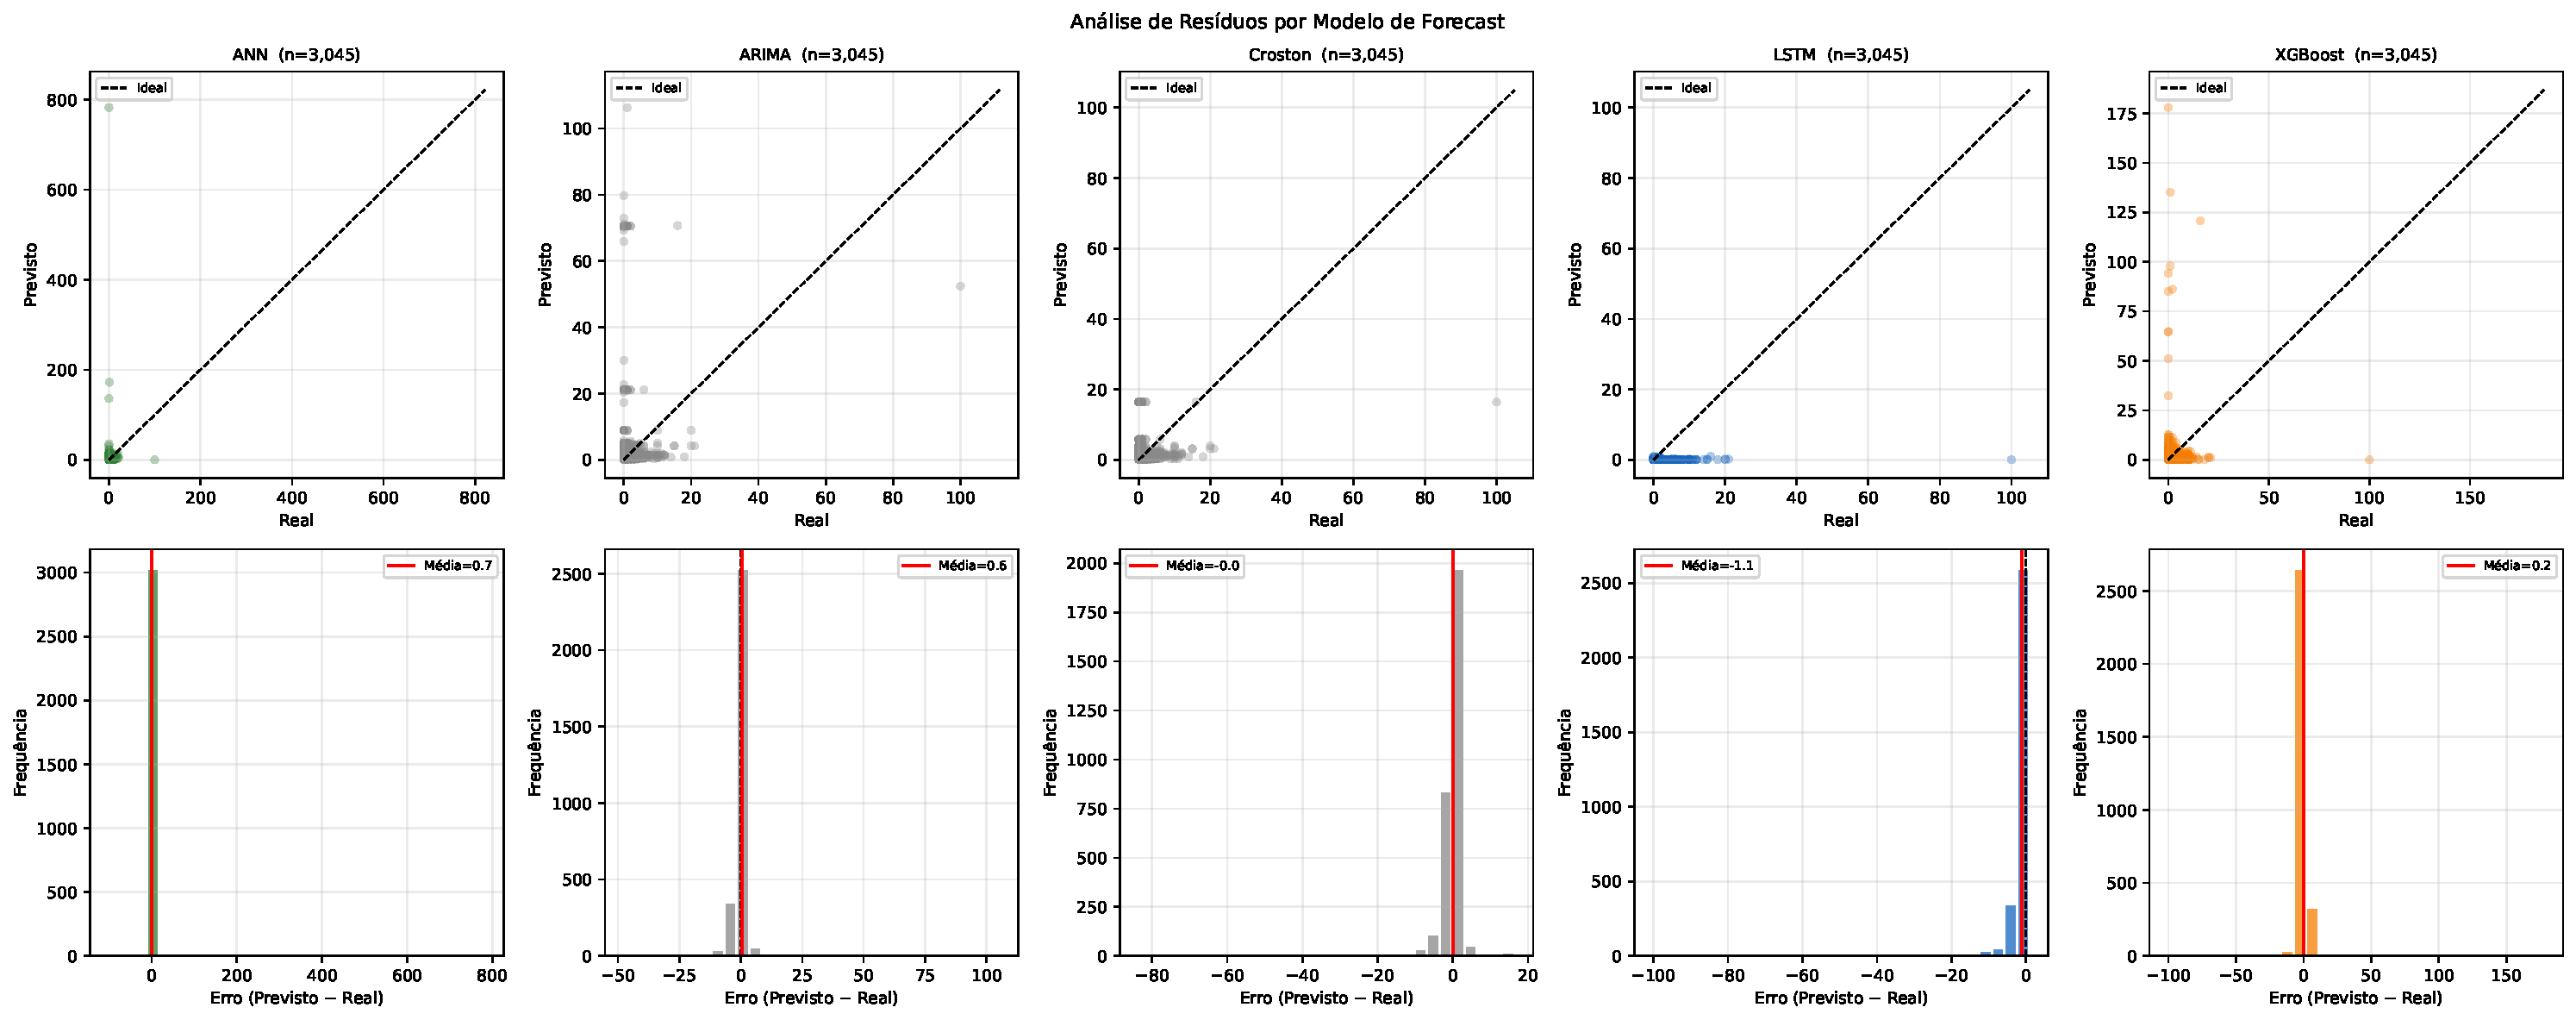
\includegraphics[width=0.80\textwidth]{../../simulation/data/08_reporting/forecast/forecast_residuals}
\caption{Distribuição dos resíduos (previsão $-$ real) por modelo sobre as 145 séries da Fase~2. O LSTM apresenta menor viés sistemático; XGBoost e ANN exibem subestimação nos picos de demanda acima do percentil~75, típica do regime \textit{Lumpy}.}
\label{fig:forecast_residuals}
\end{figure}

O módulo de caracterização de demanda produz o espaço ADI$\times$CV$^2$ apresentado na Figura~\ref{fig:adi_cv}, que confirma a predominância do quadrante \textit{Lumpy} na base atual e orienta a seleção de séries para experimentos futuros em regimes \textit{Smooth}, \textit{Erratic} e \textit{Intermittent}.

Para cada uma das 145 séries foi gerado um gráfico individual de previsão versus realizado por modelo, disponíveis em \texttt{data/08\_reporting/forecast/forecast\_vs\_actual/BA/}. A Figura~\ref{fig:forecast_vs_actual} ilustra um exemplo representativo para a loja 10533990 (produto 75792), a série de maior dificuldade da Fase~2 (ADI\,=\,$1.81$, MASE\,=\,$1.87$), com demanda média de $0.8$ unidades/ciclo e longos períodos de silêncio seguidos de picos esparsos.

\begin{figure}[ht]
\centering
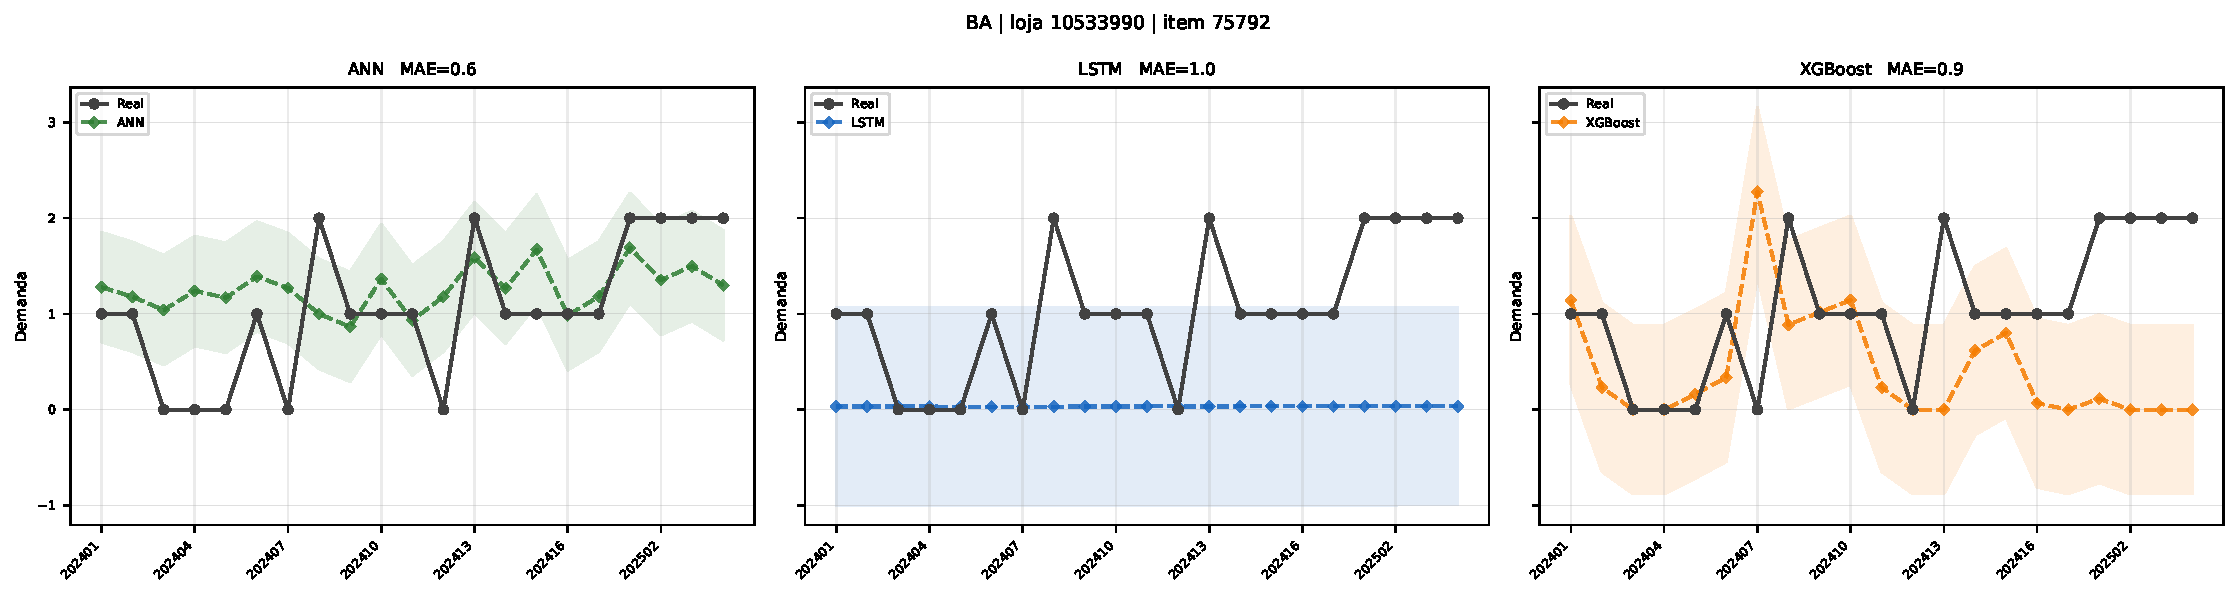
\includegraphics[width=0.85\textwidth]{../../simulation/data/08_reporting/forecast/forecast_vs_actual/BA/10533990__75792}
\caption{Previsão versus realizado para a série mais desafiadora da Fase~2 (loja 10533990, produto 75792). Os três modelos tendem a subestimar os picos de demanda, característico do regime \textit{Lumpy} com ADI elevado. O LSTM captura melhor o retorno ao zero entre os eventos positivos.}
\label{fig:forecast_vs_actual}
\end{figure}

\begin{figure}[ht]
\centering
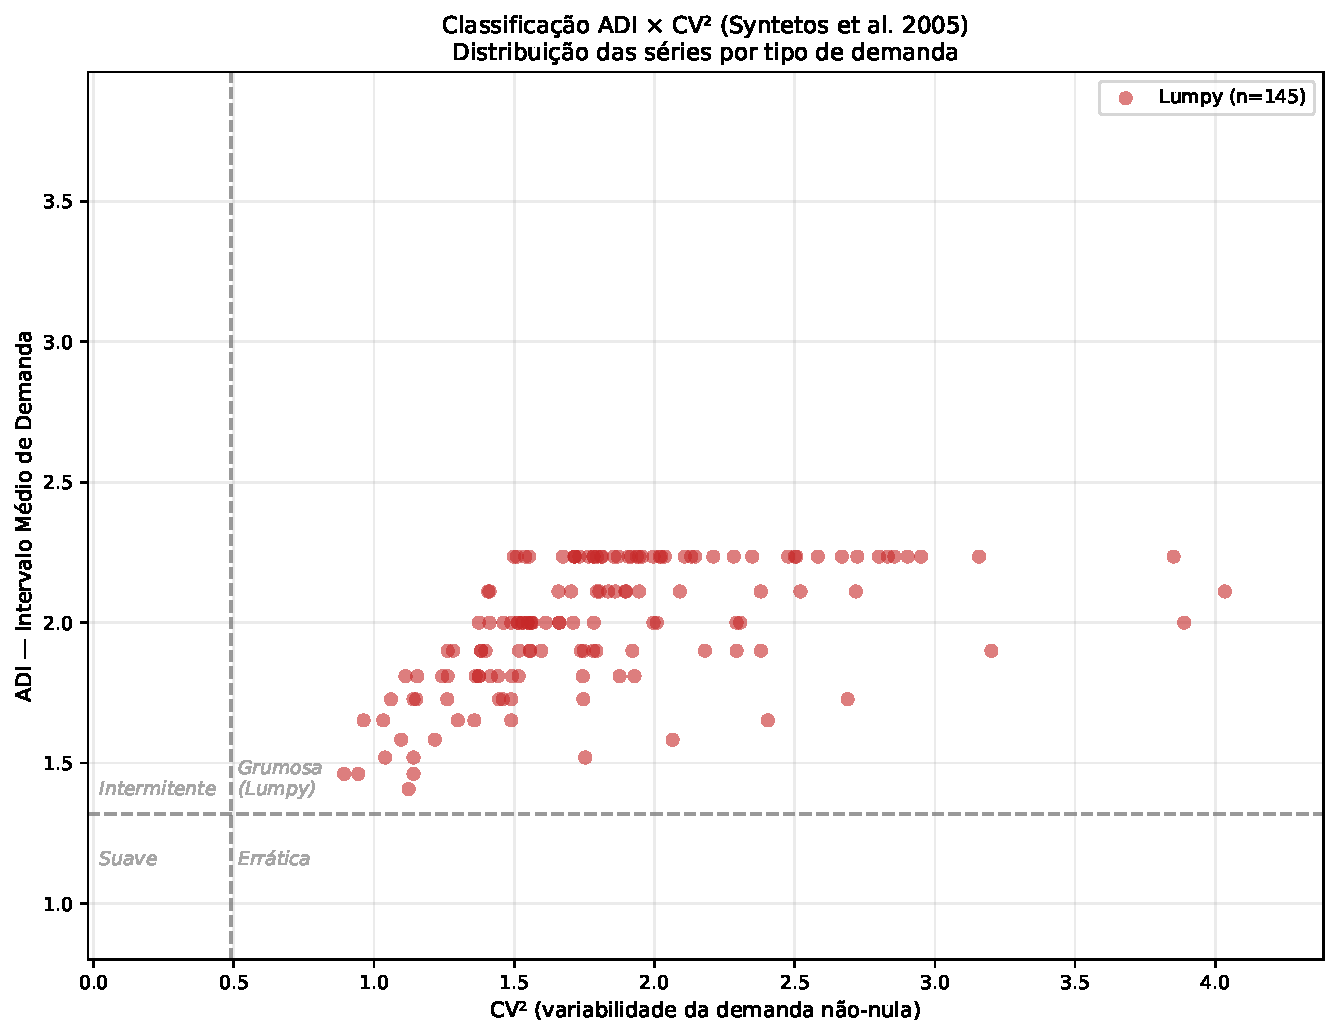
\includegraphics[width=0.68\textwidth]{../../simulation/data/08_reporting/demand/adi_cv_scatter}
\caption{Espaço ADI$\times$CV$^2$ de Syntetos-Boylan para as 145 séries da Fase~2. Linhas tracejadas: limiares $\text{ADI}=1.32$ e $\text{CV}^2=0.49$. Todas as séries encontram-se no quadrante \textit{Lumpy}.}
\label{fig:adi_cv}
\end{figure}


\section{Posicionamento em Relação à Literatura}

\begin{table}[ht]
\centering
\small
\caption{Posicionamento desta dissertação em relação aos trabalhos relacionados. \textbf{Negrito}: dimensões em que o escopo ou protocolo desta dissertação se diferencia da literatura.}
\label{tab:relwork_fase2}
\begin{tabular}{@{}lccccc@{}}
\toprule
Trabalho &
\makecell[c]{Dados\\Reais} &
\makecell[c]{CV\\(regime)} &
\makecell[c]{Políticas\\(\#)} &
\makecell[c]{Multi-\\nível} &
\makecell[c]{Indicadores\\(\#)} \\
\midrule
\citealt{Oroojlooyjadid2022BeerGameDQN} & Não & $<1$         &  3 & Sim & 2 \\
\citealt{Vanvuchelen2020PPOJointReplenishment} & Não & $<1$         &  4 & Não & 1 \\
\citealt{Gijsbrechts2022DRLInventoryMSOM}      & Não & $<1$         &  6 & Sim & 2 \\
\citealt{Yuna2023IntermittentMetaheuristics}   & Não & $>1.5$     &  2 & Não & 2 \\
\citealt{Erkayman2025MarkovInventory}          & Não & $>1.5$     &  2 & Não & 1 \\
\citealt{Liu2024HAPPO}                         & Não & $<1$         &  4 & Sim & 2 \\
\citealt{Zabraoui2025GaDQN}                   & Não & $<1$         &  7 & Sim & 3 \\
\midrule
\textbf{Esta dissertação (Fase~1)}
  & \textbf{Sim}
  & $\mathbf{2.5}$ a $\mathbf{5.4}$
  & \textbf{12}
  & \textbf{Sim}
  & \textbf{5} \\
\textbf{Esta dissertação (Fase~2)}
  & \textbf{Sim}
  & \textbf{todos os regimes}
  & \textbf{12}
  & \textbf{Sim}
  & \textbf{5 + forecast + AIPE} \\
\bottomrule
\end{tabular}
\end{table}

Os trabalhos relacionados mais próximos, \citet{Zabraoui2025GaDQN} e \citet{Yuna2023IntermittentMetaheuristics}, operam com dados sintéticos e conjuntos reduzidos de políticas. Esta dissertação avança simultaneamente em quatro dimensões: (i)~dados transacionais reais em larga escala do varejo brasileiro; (ii)~regime de demanda de alta dificuldade (CV entre 2.5 e 5.4); (iii)~benchmarking sistemático com 12 políticas e validação estatística formal; e (iv)~o módulo AIPE de seleção adaptativa de política, que aprende o mapeamento features operacionais $\rightarrow$ política ótima por série em lugar de aplicar uma política única fixa.


\section{Limitações e Trabalho em Andamento}

Os resultados da Fase~2 endereçam três das quatro limitações identificadas na Fase~1:

\begin{enumerate}
  \item \textbf{[Endereçado] Ausência de testes de significância}: as cinco replicações habilitaram os testes de Wilcoxon, Friedman e Cohen's $d$, transformando as comparações de médias em evidência estatisticamente fundada (Seção~\ref{sec:stats}).

  \item \textbf{[Endereçado] Escopo restrito}: a Fase~2 cobre 145 séries do estado da Bahia em múltiplos SKUs e lojas. A extensão aos demais estados (Pernambuco, Sergipe, Alagoas, Rio Grande do Norte) está em andamento e aguarda infraestrutura de processamento distribuído para as $\approx 10.4$ milhões de séries do dataset nacional.

  \item \textbf{[Parcialmente Endereçado] Ausência de previsão de demanda}: o módulo de previsão (LSTM, XGBoost, ANN) foi integrado e avaliado sobre as 145 séries da Fase~2. O impacto da incerteza de previsão sobre o desempenho das políticas (CTI, NS, BE) será quantificado na extensão nacional.

  \item \textbf{[Em Andamento] Avaliação in-sample}: a validação \textit{out-of-sample} com janela deslizante (\textit{walk-forward}) está implementada no módulo de previsão e será estendida ao módulo de simulação de políticas na escala nacional.
\end{enumerate}
